\documentclass[10pt]{automatisme}


\begin{document}

\begin{frame}
	\begin{minipage}{0.4\textwidth}
		Recopier le schéma ci-contre :
	\end{minipage}\hspace{0.05\textwidth}
	\begin{minipage}{0.5\textwidth}
		\begin{center}
			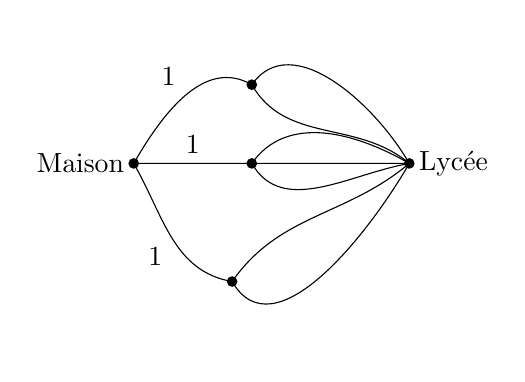
\begin{tikzpicture}[scale=0.5]
				\coordinate (Maison) at (0,0);
				\coordinate (Lycée) at (7,0);
				\coordinate (A) at (3,2);
				\coordinate (B) at (3,0);
				\coordinate (C) at (2.5,-3);
				\node[left] at (Maison) {Maison};
				\node[right] at (Lycée) {Lycée};

				\foreach \p in {Maison,Lycée,A,B,C} {
						\draw[fill=black] (\p) circle (0.12);
					}

				\draw (Maison) to[out=60,in=150] node[above left] {\correction{$1$}} (A)
				(Maison) -- node[above] {\correction{$1$}} (B)
				(Maison) to[out=-60,in=170] node[below left] {\correction{$1$}} (C);

				\draw (A) to[out=55,in=120] (Lycée)
				(A) to[out=-60,in=140] (Lycée);

				\draw (B) to[out=55,in=150] (Lycée)
				(B) -- (Lycée)
				(B) to[out=-60,in=190] (Lycée);

				\draw (C) to[out=55,in=220] (Lycée)
				(C) to[out=-60,in=240] (Lycée);
			\end{tikzpicture}
		\end{center}
	\end{minipage}

	Pour aller au lycée, Luis peut suivre un des chemins représentés ci-dessus. À chaque intersection,
	\begin{itemize}
		\item Si il y a trois rues possibles, il choisit la rue centrale (notée $C$) dans $70$\% des cas, et la rue de droite (notée $D$) dans $20$\% des cas.
		\item Si il y a deux rues possibles, il choisit la rue de gauche (notée $G$) dans $60$\% des cas.
	\end{itemize}

	\begin{enumerate}
		\item Dans tous les cas, Luis rencontre deux intersections. Ces deux épreuves sont-elles indépendantes ?
		\item Quelle est la probabilité qu'il prenne deux fois à droite pour aller au lycée ?
		\item Quelle est la probabilité qu'il ait pris au moins une fois à gauche pour aller au lycée ?
	\end{enumerate}
\end{frame}

\end{document}